\documentclass[12pt, unicode]{beamer}
\usepackage{luatexja}
\usepackage{xurl}
\usepackage{tikz}
\usetikzlibrary{
  intersections,
  calc,
  arrows.meta,
  angles,
  quotes,
  graphs,
  positioning
}
\usetheme{metropolis}
\usepackage[absolute,overlay]{textpos}
\title{情報発酵、始めませんか?}
\author{淡中圏}
\date{}

\begin{document}

\frame{\titlepage}

\begin{frame}

みなさん、眠っているファイル、ありませんか?

ずっと使っていないファイル、存在すら忘れていたファイル、ファイル名を見てもなんだかわからないファイル。

\end{frame}
\begin{frame}

\Large
\centerline{そんなファイルを有効利用してみませんか?}

\end{frame}

\begin{frame}

みなさんのパソコンのディスク、もしかして半分以上使われていないんじゃないですか?

今時HDDもSSDも安くなったので、十分な余裕を持っているんじゃないかと思いますが、だからこそ大半は空いていますよね。

\end{frame}
\begin{frame}

\Large
\centerline{その使っていない容量、有効利用しませんか?}

\end{frame}

\section{我々の技術}

\begin{frame}

我々の開発した新しい技術は\textbf{「データの発酵」}です。

これには長年のコンピュータウィルスに対する研究が活かされています。

\end{frame}
\begin{frame}

我々はこれまで、コンピュータウィルスからみなさんのデータを守るためのの研究に邁進し続けていました。

しかし、遺伝的アルゴリズムや遺伝的プログラミングなどの進化型計算の手法を取り入れた現代のコンピュータウィルスは、すでに完全な対策の不可能な存在と化しています。

そこで我々は、これらのコンピュータウィルスへの対処は、旧来の人工物への対処法ではなく、実際のウィルスに対するのと同様の、自然の生物への対処法に近くするべき、と考えました。

{\Large
\centerline{つまり「共存共栄」です。}
}
\end{frame}

\begin{frame}

そこで、サンドボックス化された環境を多数用意して、そこでさまざまなウィルスを培養する研究をしました。

それぞれのサンドボックスには、
ドキュメント、
表計算、
プレゼンテーション、
画像、
音声、
動画、
などなど特色あるファイルを多数置きました。

\end{frame}
\begin{frame}

もちろん最初のうちは全てのウィルスがファイルを壊してしまいました。

しかし、超並列計算で何世代も我慢強く観察することにより、その中からファイルを壊さず、むしろファイルをよりよくしてくれるウィルスを選別することが可能になりました。

そしてそれらのウィルスがより増えて、そうでないウィルスは減っていくように影響を与えることにより、
人類に役立つようにコンピュータウィルスを\textbf{進化}させていくことが可能になったのです。

\end{frame}

\begin{frame}

例えばある種のウィルスは低解像度の画像や動画を高解像度化します。

\begin{figure}[htbp]
  \begin{minipage}[b]{0.4\linewidth}
    \centering
    
\includegraphics[keepaspectratio, scale=1.2]{pic1_resize.jpg}
  \end{minipage}
  \begin{minipage}[b]{0.18\linewidth}
    \begin{tikzpicture}
      \draw[transparent] (0,0)--(0,2);
      \draw[->](0,2)--(2,2);
    \end{tikzpicture}
  \end{minipage}
  \begin{minipage}[b]{0.4\linewidth}
    \centering
    
\includegraphics[keepaspectratio, scale=0.15]{pic1.jpg}
  \end{minipage}
  \caption{解像度が上がっている}
\end{figure}

\end{frame}
\begin{frame}

別のウィルスはよくない構図で撮られた写真をもっと良い構図の写真へと変換します。

\begin{figure}[htbp]
  \begin{minipage}[b]{0.4\linewidth}
    \centering
    
\includegraphics[keepaspectratio, scale=0.15]{pic3.jpg}
  \end{minipage}
  \begin{minipage}[b]{0.18\linewidth}
    \begin{tikzpicture}
      \draw[transparent] (0,0)--(0,2);
      \draw[->](0,2)--(2,2);
    \end{tikzpicture}
  \end{minipage}
  \begin{minipage}[b]{0.4\linewidth}
    \centering
    
\includegraphics[keepaspectratio, scale=0.15]{pic2.jpg}
  \end{minipage}
  \caption{下からのおかしな構図で撮られた写真を正面からの構図に変換している}
\end{figure}

\end{frame}
\begin{frame}

メールや書類の文面を添削するウィルスも存在しますし、表計算の数式の間違いを修正してくれるウィルスや、音の入っていないアニメーションに音楽やセリフを入れてくれるウィルスも存在します。

\begin{figure}[htbp]
  \begin{minipage}[b]{0.2\linewidth}
    
\includegraphics[keepaspectratio, scale=0.1]{pic4.png}
  \end{minipage}
  \begin{minipage}[b]{0.1\linewidth}
    \begin{tikzpicture}
      \draw[transparent] (0,0)--(0,0.25);
      \draw[->](0,0.25)--(1,0.25);
    \end{tikzpicture}
  \end{minipage}
  \begin{minipage}[b]{0.2\linewidth}
    
\includegraphics[keepaspectratio, scale=0.1]{pic5.png}
  \end{minipage}
  \begin{minipage}[b]{0.1\linewidth}
    \begin{tikzpicture}
      \draw[transparent] (0,0)--(0,0.25);
      \draw[->](0,0.25)--(1,0.25);
    \end{tikzpicture}
  \end{minipage}
  \begin{minipage}[b]{0.2\linewidth}
    
\includegraphics[keepaspectratio, scale=0.1]{pic6.png}
  \end{minipage}
  \caption{チラシのデザインをウィルスが徐々に改善している様子}
\end{figure}



\end{frame}

\begin{frame}

これはつまり、今までのウィルスによるデータの破壊が自然界における細菌や菌類による「腐敗」であるとするならば、\textbf{「発酵」}に当たる現象だと言えます。

\end{frame}

\begin{frame}

もちろんこれらの仕事は全て通常の人工知能にも可能です。

通常の人工知能との違いはその高い\textbf{進化性}です。

無数のコンピュータウィルスがコンピュータ内で覇権を争うことにより、こちらが与えていない情報を勝手に探し求め吸収し、通常の人工知能では考えられない速度で自動的に進化します。

通常の人工知能との違いは生存競争による強い\textbf{生存欲求}です。
それにより、当初は予測もしなかった挙動をこれらが示すことを我々は何度も観察してきました。

\end{frame}

\begin{frame}

例えば、我々のコンピュータウィルスで発酵させたファイルはただ単にクオリティが高くなっただけではありません。
それは他のコンピュータウィルスの破壊に対する強い\textbf{ロバスト(頑健)性}を示すようになりました。

\end{frame}
\begin{frame}

\vspace{2\baselineskip}

つまり、一度我々のコンピュータウィルスで発酵して仕舞えば、他のコンピュータウィルスに破壊される(つまり腐敗する)心配はほぼなくなり、
セキュリティ的にも安心なのです。
これは発酵食品が腐敗しにくくなり長持ちする現象と似ています。

\begin{figure}[htbp]
  \begin{minipage}[b]{0.8\linewidth}
    \centering
    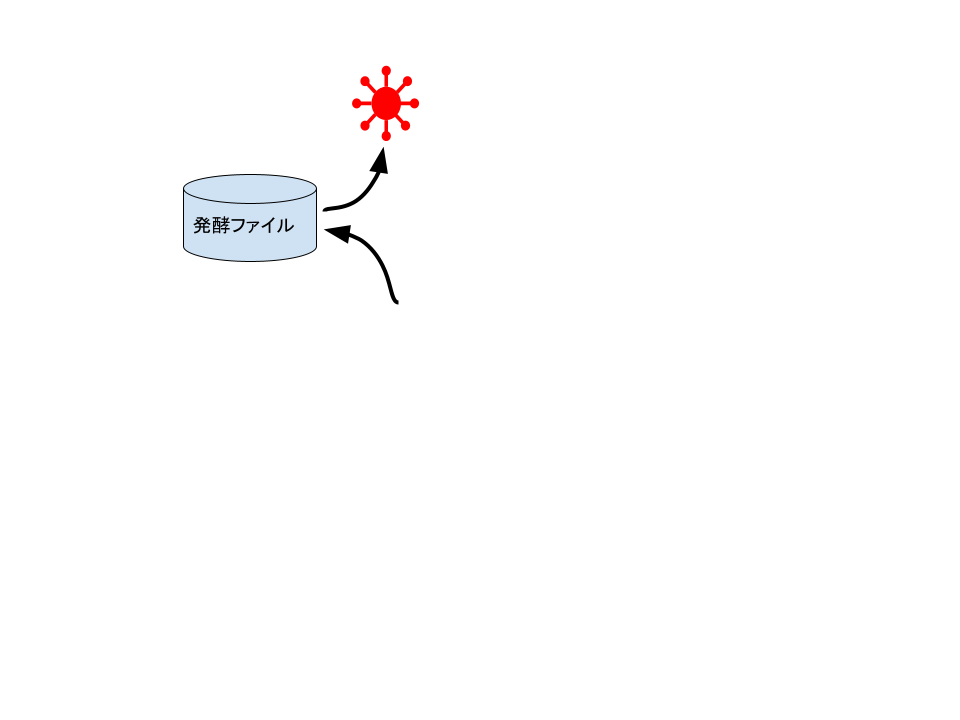
\includegraphics[keepaspectratio, scale=0.3]{fig2.png}
  \end{minipage}
\end{figure}


\end{frame}

\section{我々が提供するソリューション}

\begin{frame}

我々が皆様にご提供するソリューションは、皆様のコンピュータの空きスペース内にこれらのコンピュータウィルスを培養するサンドボックスを構築することです。

ウィルスたちは、空きスペース内にあるファイルの痕跡(皆さんがコンピュータ内で削除したファイルの内容の断片はすぐに消えるわけでなく、新しいファイルで上書きされるまで空きスペース内に存在します)を発酵させます。

それによって、ウィルスたちは皆様のコンピュータ内に多く存在するファイルの種類を学び、そこに生息するのに最適な状態に素早く進化します。
また我々のアプリも、それらのウィルスに何が可能かを把握し、皆様に提供することができます。

\end{frame}

\begin{frame}

\vspace{1\baselineskip}

これは、丁度家庭において生ごみなどを微生物に分解させて堆肥にすることと同じです。

例えこのシステムを導入したとしても、皆様のコンピュータの空きスペースはほとんど減りません。

ウィルスが普段活動している空きスペースはいつでも使用可能です。

\begin{figure}[htbp]
  \begin{minipage}[b]{0.8\linewidth}
    \centering
    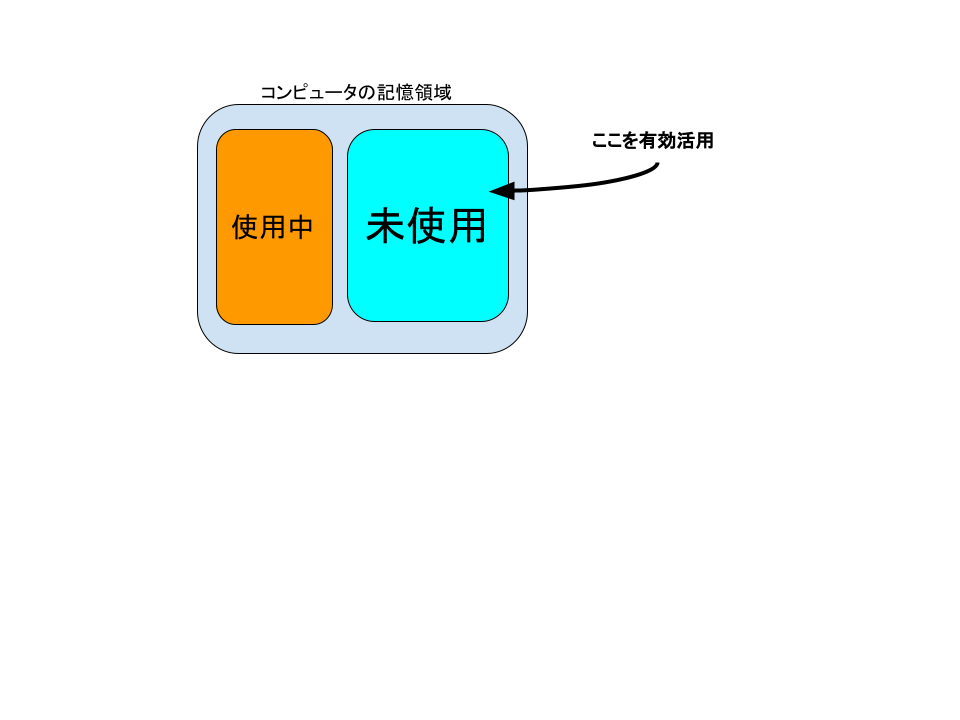
\includegraphics[keepaspectratio, scale=0.3]{fig1.png}
  \end{minipage}
\end{figure}

\end{frame}

\begin{frame}

そして学習されたウィルスを使って、さまざまなファイルを素早く発酵させることができるようになるのです。

また、使っていないけど消していないファイルを発酵する許可を与えれば、それらの中から有用になりそうなファイルをシステムが皆様に提案することも可能です。

\end{frame}

\begin{frame}

こうすることで、普段使われていないディスク容量やCPUを最大限に有効活用することができます。

これはまさに\textbf{SDGsの時代}、\textbf{循環型社会}の申し子と言っていいでしょう。

\end{frame}

\begin{frame}{始めるなら今です}

ご興味がある岡田は下のリンクをクリックしてください。
我々が育てたコンピュータウィルスが早速皆様のコンピュータ内で活動を始めます。

{\color{blue}
\href{https://google.com}{\underline{発酵を始める}}
}

\end{frame}

\end{document}
